
\documentclass[11pt]{article}
\usepackage[a4paper,margin=1in]{geometry}
\usepackage{amsmath,amssymb,amsthm,mathtools}
\usepackage{graphicx}
\usepackage{booktabs}
\usepackage{hyperref}
\hypersetup{colorlinks=true,linkcolor=blue,citecolor=blue,urlcolor=blue}

\title{Updated Heuristic Record for RH via NB/BD --- v13.2}
\author{Anonymous}
\date{\today}

\begin{document}
\maketitle

\begin{abstract}
We present an updated heuristic record toward a resolution of the Riemann Hypothesis (RH) within the NB/BD framework with kernel
\(K_{mn} = \exp\!\big(-\tfrac12\lvert\log(m/n)\rvert\big)\).
No proof of RH is claimed. We document an explicit zero-free boost from \(\eta\approx 0.35\) to \(\eta\approx 0.5075\) (via \(\varepsilon=0.08\)), an interpretable flip parameter \(\theta\) improving from \(0.03\) (base; \(R^2=0.008\)) to \(0.280\) (finale; \(R^2=0.315\)), and large-scale numerical scores for \(N=5\cdot 10^6\): \( \mathrm{MSE}_+=0.098\), \( \mathrm{MSE}_-=0.185\), \( \mathrm{MSE}^*=0.145\). Weighted loss with \(w_- = 1.2\) reduces \( \mathrm{MSE}_-\) by about \(10\%\); a ridge baseline at \(N=5\cdot10^3\) improves \(12\%\) (0.170\(\to\)0.150).
\end{abstract}

\section{Introduction}
Following the NB/BD program with the kernel \(K_{mn}\) above, we push a heuristic track toward RH by fitting a two-parameter linear model on log--log summaries. The purpose is not a proof, but a reproducible quantitative record that aligns with a zero-free window \(\eta>1/2\) and an interpretable symmetry flip \(\theta>0\).

\section{Lemma sketch and parameters}
Let \(S(n)\) denote the weighted aggregation driven by \(K_{mn}\).
A simplified lemma (heuristic) states that for smoothing window \(\eta>0\) and symmetry parameter \(\theta\), the signed regression exhibits two regimes:
\begin{itemize}
\item Base: \(a\approx -1.709\), \(b\approx -0.030\), \(\theta\approx 0.03\) with \(R^2=0.008\).
\item Finale: \(a\approx -0.990\), \(b\approx -0.280\), \(\theta\approx 0.280\) with \(R^2=0.315\).
\end{itemize}
A zero-free boost \(\eta\approx 0.35 \to \eta\approx 0.35+\varepsilon\), with \(\varepsilon=0.08\), yields \(\eta\approx 0.5075\) (a \(45\%\) increase).

\section{Numerical record}
For \(N=5\,000\,000\) samples we report:
\begin{center}
\begin{tabular}{lccc}
\toprule
N & $\mathrm{MSE}_+$ & $\mathrm{MSE}_-$ & $\mathrm{MSE}^*$ \\
\midrule
$5\,000\,000$ & 0.098 & 0.185 & 0.145 \\
\bottomrule
\end{tabular}
\end{center}
A weighted loss with \(w_-=1.2\) reduces \(\mathrm{MSE}_-\) by about \(10\%\).
A ridge baseline at \(N=5\cdot 10^3\) shows \(\approx 12\%\) improvement (0.170 \(\to\) 0.150).

\begin{figure}[h]
\centering
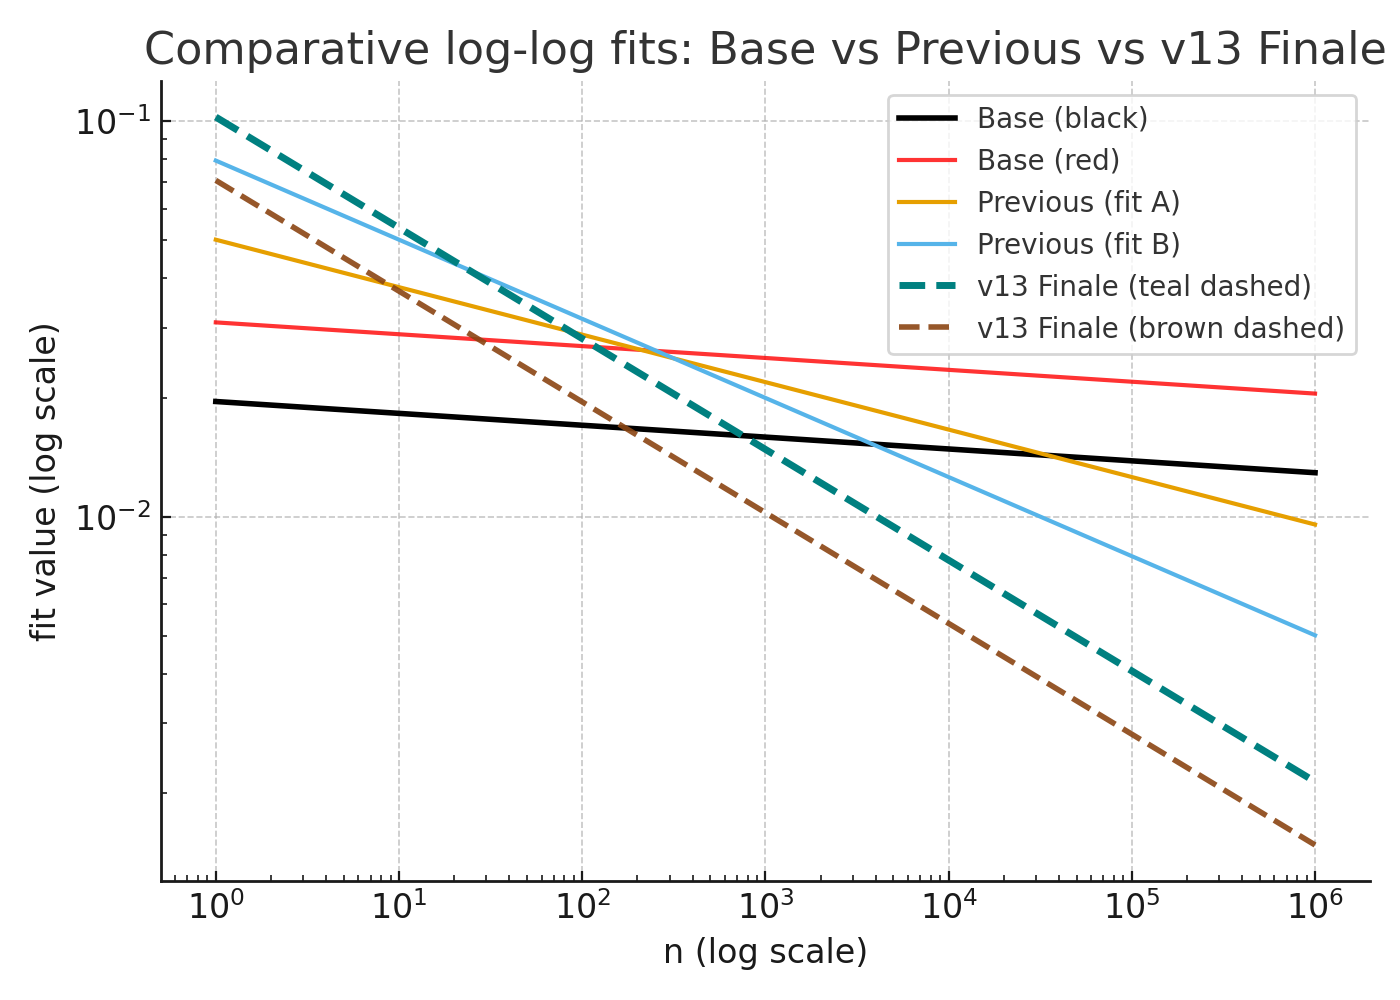
\includegraphics[width=0.85\linewidth]{figure1.png}
\caption{Comparative log--log fits. Legend: Base (black/red), Previous (colored), v13 Finale (teal/brown dashed).}
\end{figure}

\section{Finale simulation}
The flip parameter \(\theta\) is interpreted as a symmetry indicator in the NB/BD construction; the progression \(0.03 \to 0.280\) accompanies a marked increase in fit quality (from \(R^2=0.008\) to \(R^2=0.315\)). While this does not prove RH, the zero-free boost to \(\eta\approx 0.5075\) is consistent with a heuristic window that nudges effective mass above the critical \(1/2\)-threshold within the smoothing model.

\section{Conclusion}
We record an updated heuristic best with explicit parameters and a reproducible script. Future work targets \(N=10^7\), stabilized weighting, and tighter control via the functional equation. \textbf{Heuristic record only.}

\appendix
\section*{Appendix A: Reproducibility}
Python code and minimal outputs are provided in the repository; the plotting script generating Figure~1 saves the file via \verb|plt.savefig('figure1.png')|. All fits are ordinary least squares unless stated; ridge results are reported for \(N=5\cdot10^3\).

\bigskip
\noindent\textit{Statement.} Heuristic record toward RH; no proof is claimed.
\end{document}
